\begin{table*}[ht]
\footnotesize
\centering
\begin{tabular}{llccc}
\toprule
& \textbf{Train examples} & \textbf{HANS} & \textbf{MNLI} & \textbf{Avg.}  \\
\midrule
\small{1} & All & 58.3 & \textbf{84.5} & 71.4        \\
\midrule
\small{2} & \bertbase forgettables $_{\balancedbert}$   & 48.8                     & 38.9                         & 43.9\\
\small{3} & \hspace{0.1cm} Random $_{\balancedbert}$ & 51.9                   & 75.7                         & 63.8\\
\small{4} & BiLSTM forgettables $_{\balancedlstm}$ & 54.0                     & 66.8                         & 60.4 \\
\small{5} & \hspace{0.1cm} Random $_{\balancedlstm}$ & 51.1                   & 79.0                         & 65.1\\
\small{6} & BoW forgettables $_{\balancedbow}$    & 54.1                     & 68.3                         & 61.2 \\
\small{7} & \hspace{0.1cm} Random $_{\balancedbow}$ & 53.9                   & 79.6                         & 66.8\\
\midrule
&\emph{Additional stage of finetuning} \\
\small{8} & All + \bertbase forgettables   & 70.8                     & 81.8                         & 76.3  \\
\small{9} & All + BiLSTM forgettables &  {73.6}                     & 82.4             & {78.0} \\
% \small{10} & \hspace{0.1cm} All + Random $_{\balancedlstm}$       & 60.9                     & 84.4                         & 72.7  \\
\small{10} & All + BoW forgettables    & \textbf{73.7}                     & 82.4             & \textbf{78.1} \\
\small{11} & \hspace{0.1cm} All + Random $_{\balancedbow}$       & 60.6                     & 84.1                         & 72.35  \\
\midrule
&\emph{Additional stage of finetuning (avg${_{\pm std}}$)} \\
\small{8} & All + \bertbase forgettables   
& $67.4_{\pm 2.47}$                     & $82.0_{\pm 0.25}$                         &   \\
\small{9} & All + BiLSTM forgettables 
&  $69.9_{\pm 2.24}$  & $82.7_{\pm 0.25}$             &  \\
\small{11} & All + BoW forgettables    & $70.4_{\pm 2.10}$                     & $82.5_{\pm 0.25}$             &  \\
\midrule
&\emph{From~\citet{clark2019dont}} & & & \\
\small{12} & All & 62.4 & 84.2 & 73.3 \\
\small{13} & All (reweight) & 69.2 & 83.5 & 76.4 \\
\small{14} & Learned Mixin & 64.0 & 84.3 & 74.2\\
\midrule
&\emph{From~\citet{mahabadi2019simple}} & & &  \\
\small{15} & Product of Experts & 66.5 & 84.0 & 75.3     \\
\midrule
&\emph{From~\citet{he2019unlearn}} & & &  \\
\small{15} & DRiFt-HYPO & 67.1 & 84.3 & 75.7     \\
\midrule
&\emph{From~\citet{linzen2019right} and \citet{Nangia_2019}} & & &  \\
\small{16} & Estimated MTurks & 76.0 & 92.0 & 84.0 \\
\bottomrule
\end{tabular}
\caption{Results of \bertbase model trained on different sources of training examples. For each line, the accuracy of the corresponding model is shown on MNLI dev and HANS and the average of the two.  
Line 1 replicates the original \bertbase result~\citep{devlin2018bert}.
% We denote with $\Delta$ the absolute improvement with respect to the standard setting of fine-tuning on all the MNLI examples (first row). 
Lines from 2 to 7 correspond to finetuning only on subsets of MNLI data. The third block of results (lines from 8 to 11) corresponds to first finetuning \bertbase on the entire MNLI data and then performing an additional finetuning stage on selected examples. We also compare performance to the recent baselines of \newcite{clark2019dont} (lines 12 to 14) and \newcite{mahabadi2019simple} (line 15). They obtain slightly higher results for their base model~\textrm{All} but our best model outperforms theirs.}
\label{tab:twoclass}
\end{table*}

\begin{table*}[]
\small
\centering
\begin{tabular}{lccccccc}
\toprule
\textbf{Model} & \multicolumn{3}{c}{\textbf{Entailment}} & & \multicolumn{3}{c}{\textbf{Contradiction}} \\
& \emph{All}    & \emph{High}  & \emph{Low} & & \emph{All}     & \emph{High}    & \emph{Low} \\
\midrule
All & \textbf{84.1}   & \textbf{90.2}   & \textbf{75.8}  & & 84.7    & 85.4    & \textbf{84.3} \\
All + BiLSTM forgettables & 77.9   & 82.6   & 71.5  & & \textbf{85.0}      & \textbf{87.0} & 84.0  \\   
\bottomrule
\end{tabular}
\caption{Fine-grained accuracy results of \bertbase on MNLI dev set before and after finetuning
on forgettables. 
We split the evaluation set into High ($>$ mean) and Low ($<$ mean) word-overlap examples,
where word-overlap is measures under Jaccard Index between hypothesis and premise. 
Finetuning hurts \ent{} results in both High and Low but improves \nent{} on High.
This is in line with the fine-grained results of HANS depicted in Figure \ref{fig:fine_eval_baselines} where all examples have High word-overlap.}
\label{fine_mnli}   
\end{table*}

\begin{figure}[t]
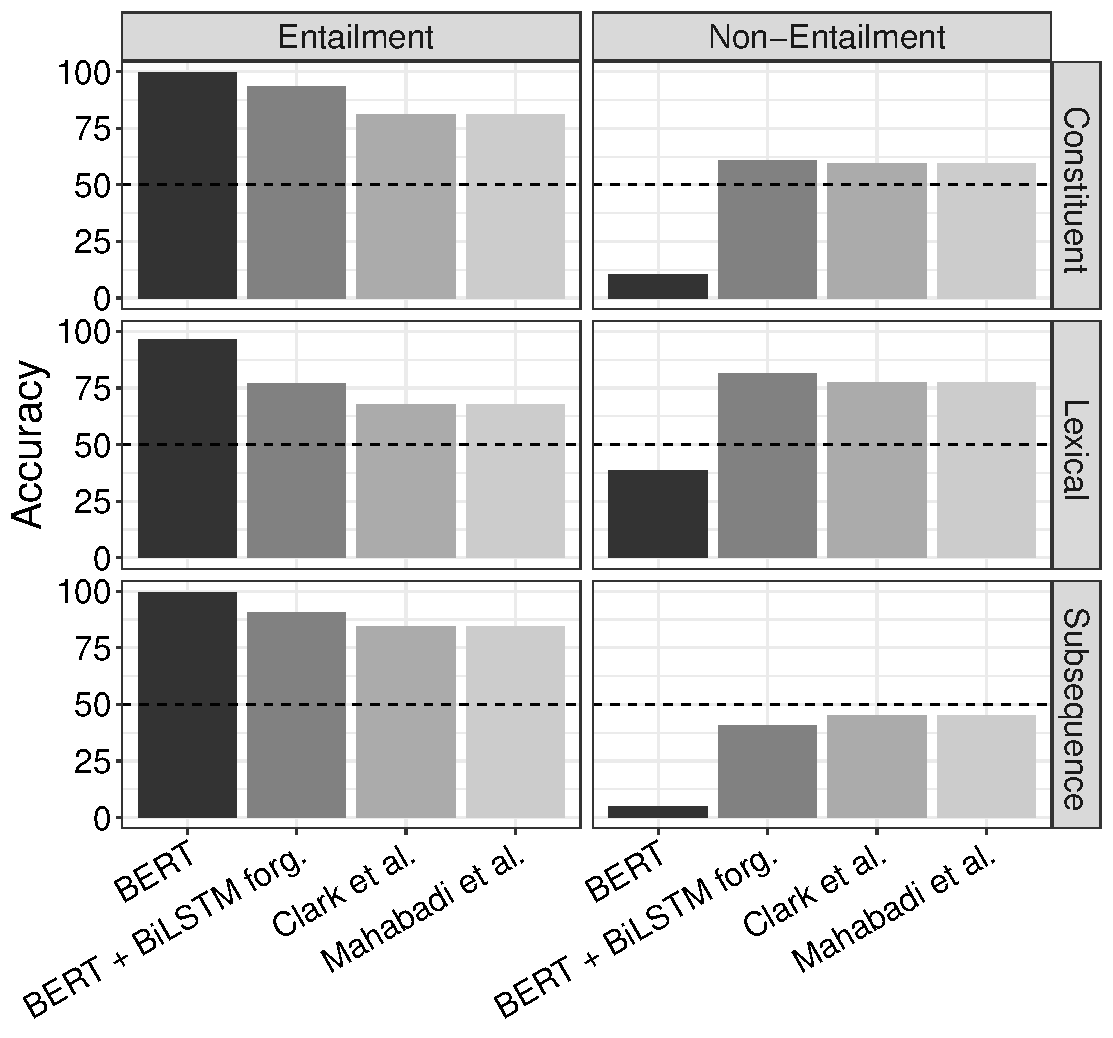
\includegraphics[scale=0.42]{figures/heuristic_plot.pdf}
\caption{Performance of tested models versus the baselines for ``entailment'' and ``non-entailment'' categories and for each heuristic present in the HANS test set. Our approach seems to better retain performance of the entailment category while still increasing accuracy over the baselines of the non-entailment category, albeit to a smaller extent.}
\label{fig:fine_eval_baselines}
\end{figure}


\iffalse
\begin{table}[ht]
\small
\caption{Results of \bertlarge model trained on different sources of training examples.}
\small
\label{tab:bertlarge}
\centering
\begin{tabular}{lccc}
\toprule
\textbf{Train examples} & \textbf{HANS} & \textbf{MNLI} & \textbf{Avg.}  \\
\midrule
All & 72.3 & 86.4 &  79.3 \\
\midrule
\emph{Additional stage of finetuning} & & &\\
All + BoW forgettables & 77.3 & 85.5 & 81.4 \\
All + BiLSTM forgettables & \underline{77.5} & \underline{85.5} & \underline{81.5} \\
\bottomrule
\end{tabular}
\end{table}
\fi

\begin{table*}[ht]
\small
\centering
\begin{tabular}{lcccccc}
\toprule
\textbf{Model} & \multicolumn{2}{c}{\textbf{HANS}} & \multicolumn{2}{c}{\textbf{MNLI}} & \multicolumn{2}{c}{\textbf{Avg.}}  \\
& \emph{base} & \emph{large} & \emph{base} & \emph{large} & \emph{base} & \emph{large} \\
\midrule
BERT & 58.3 & 72.3 & 84.5 & 86.4 & 71.4 & 79.3 \\
BERT + BoW forgettables & 73.7 & 77.3 & 82.4 & 85.5 & 78.1 & 81.4 \\
BERT + BiLSTM forgettables & 73.6 & 77.5 & 82.5 & 85.5 & 78.3 & 81.5 \\
\midrule
XLNET & 63.9$_{\pm 3.0}$ & $76.1_{\pm 2.7}$ & $86.5_{\pm 0.29}$ & 89.7$_{\pm 0.1}$ & & \\
XLNET + BoW forgettables & 73.0 & 85.0 & 84.3 & 88.2 & \\
XLNET + BiLSTM forgettables & 75.1 & 86.8 & 85.5 & 87.8 & &  \\
%\midrule
%Roberta & 46.3 & 50.2 & 87.9 & 89.9 &  & 84.15 \\
%Roberta + BoW forgettables & & & & & \\
%Roberta + BiLSTM forgettables & & & & & & \\
\bottomrule
\end{tabular}
\caption{Results of the \emph{base} and \emph{large} version of various recent NLU models trained on different sources of training examples.}
\label{tab:bertlarge}
\end{table*}



Our main results are presented in Table~\ref{tab:twoclass}.

\paragraph{Forgetting Statistics} Table \ref{tab:forg_stats} shows the number of forgettable examples before and after balancing for BoW, BiLSTM and BERT on MNLI. It is worth noting that the larger the model, the fewer the forgettable examples. The performance of the models on the development set of MNLI is also included, and appears negatively correlated to the number of forgettable examples. Figure~\ref{fig:forgcount-freq} displays the distribution of forgetting events for each model on MNLI, showing in particular the significant number of examples never learnt by our weak baselines.

\paragraph{Training on Forgettables} Lines 2 to 5 report results of fine-tuning BERT on different subsets of the MNLI dataset. This setting aligns with the setting presented in~\citet{toneva2018empirical} where the authors show that, in multiple image classification tasks, the same generalization performance can be obtained by training a model initialized randomly on its own forgettable examples. Our results suggest that this behavior may be task and/or architecture dependent: in our setting, training only forgettable examples particularly affects generalization performance on MNLI. The most extreme drop in performance is observed when BERT is only fine-tuned on its own forgettable examples (line 2) achieving an accuracy of 38.9\%. Training on BiLSTM (line 4) or BoW forgettables (line 6) examples causes a lesser drop in accuracy on MNLI although still noticeable. One of the possible reasons of the dramatic performance loss observed in line 2 is that BERT forgettables are significantly fewer than the counterparts from weaker baselines. 
In order to rule out this hypothesis, we train on a random subset of examples of the same size (\balancedbert, line 3). These results suggest that there is an intrinsic difficulty in BERT forgettables that deserves to be investigated in the future.
To some extent, this is also the case for BiLSTM and BoW forgettables (lines 4 and 6), when comparing to random samples with the same size (lines 5 and 7).

\paragraph{Additional Fine-Tuning} Lines 8-11 report the results obtained by fine-tuning a pretrained model on the set of forgettables, as described in Section \ref{sec:fine_tune}. The results confirm that slightly biasing the model towards hard examples improves robustness at a slight (albeit noticeable) drop in MNLI accuracy. 
Our best model is obtained by using the BoW forgettable examples (line 9) achieving an accuracy of 73.6\% on HANS (max over 3 seeds, mean 73.7\% $\pm$ 0.5\%)
which constitutes a +15.7\% absolute improvement with respect to the base model in line 1 and +4.8\% and +7.5\% with respect to the concurrent models of \newcite{clark2019dont} and \newcite{mahabadi2019simple}. 
Results on line 10 confirm that the forgettables examples identified by BiLSTM are responsible for the improvement: fine-tuning on the same number of randomly chosen examples leads to a much smaller increase. 
Fine-tuning on BoW forgettables (line 11) is also comparable to BiLSTM forgettables (line 9).
% This shows that the choice of the weak model does not seem to matter and therefore prior knowledge about the dataset biases is not required.
An additional observation is that BERT forgettables provide less improvement in robustness than BiLSTM or BoW. 
We hypothesize that this is due to the smaller size of the BERT forgettables compared to BiLSTM or BoW.
% This seems to align with our hypothesis that weaker baselines capture simpler explanations in the dataset.

\textcolor{red}{NEED TO COMMENT ON TABLE 3. We also show the detailed results of HANS based on its three different heuristics for our best performing model (line 9) in Figure \ref{fig:fine_eval_baselines}. 
To give an example of how the various models perform, we retrieved the nearest neighbors of a given HANS example (see Appendix, Table \ref{tab:NNs}).}



\paragraph{Robustness of XLNET and larger models}
\textcolor{red}{\citet{yang2019xlnet} recently introduced XLNET, a transformer-based language model outperforming BERT in standard benchmarks. We applied our evaluation procedure to XLNET and report the results in Table \ref{tab:bertlarge}. \xlnetbase reaches 63.9\% on HANS. After fine-tuning on BiLSTM forgettables, we see an increase of +11.2\%; our method seems to transfer to other architectures.}

\textcolor{red}{Perhaps more interesting, is the effect of using even bigger models. A growing body of literature suggests that increasing the capacity of deep networks results in better generalization \cite{belkin2018reconciling,deepdouble}. These results usually assume no distribution shift between train and test sets. We investigate here whether robustness to the distribution shift studied in this paper may appear ``for free'' in models with a larger number of parameters. To that end, we apply our method to the ``large'' version of BERT and XLNET, \bertlarge and \xlnetlarge, which 
achieve very strong performance on the MNLI dataset~\cite{devlin2018bert,yang2019xlnet}. Results are also shown in Table~\ref{tab:bertlarge}. We see that the large versions generalize on HANS significantly better than their base counterparts (e.g. 76.1\% vs 63.9\% for XLNET), confirming -- in this setting -- that larger models seem more robust. We also observe a significant improvement in performance as a result of finetuning on BiLSTM forgettables, supporting the applicability of the method to larger architectures. In particular, \xlnetlarge fine-tuned on BiLSTM forgettables shows a +10.7\% increase in performance, reaching an impressive 86.8\%!}

\iffalse
\begin{table*}[t]
    \centering
\setlength{\tabcolsep}{4pt}
\begin{tabular}{lcrrrrrrr}
\toprule
\multirow{2}{*}{Training examples} 
&
& \multicolumn{2}{c}{lexical} & \multicolumn{2}{c}{subseq} & \multicolumn{2}{c}{const} \\
     \cmidrule(lr){3-4} \cmidrule(lr){5-6} \cmidrule(lr){7-8}
     & overall 
            & \ent            & \nent           & \ent            & \nent           & \ent             & \nent \\
\midrule
All  & 58.3     
& \bt{0.0}{96.3} & \bt{0.0}{38.4} 
& \bt{0.0}{99.6} & \bt{0.0}{4.7} 
& \bt{0.0}{99.7} & \bt{0.0}{10.6} \\
All + finetuning on BiLSTM forgettables & 73.6   
& \bt{0.0}{76.9} & \bt{0.0}{81.6} 
& \bt{0.0}{90.6} & \bt{0.0}{40.8} 
& \bt{0.0}{93.3} & \bt{0.0}{60.8} \\
\midrule
\newcite{mahabadi2019simple} & 66.5
& \bt{0.0}{93.5} & \bt{0.0}{61.7} 
& \bt{0.0}{96.3} & \bt{0.0}{19.2} 
& \bt{0.0}{98.4} & \bt{0.0}{30.2} \\
\newcite{clark2019dont}  & 69.2
& \bt{0.0}{67.9} & \bt{0.0}{77.4} 
& \bt{0.0}{84.3} & \bt{0.0}{44.9} 
& \bt{0.0}{81.0} & \bt{0.0}{59.6} \\
\bottomrule
\end{tabular}
\caption{Accuracy of the entailment (\ent) and non-entailment (\nent) classes on HANS for three heuristics:
    lexical overlap (lexical), subsequence overlap (subseq), and constituent overlap (const).
}
\label{tab:hans-detailed}
\end{table*}
\fi